\subsection{Graphen}
Ein Graph wird definiert als eine Menge von Knoten und Kanten sowie deren Struktur und Anordnung.
Aus der Spezifikation der Map unseres Rennspiels lässt sich ein ungerichteter Graph mit 30x20 Knoten erstellen (siehe \autoref{fig:graphMaschen}).\newline

Maschen?\newline
Auch diagonal verbunden.\newline
Alle Spielknoten werden zunächst initial erzeugt.
Diese Spielknoten können anschließend mit Kanten verbunden werden (siehe \autoref{fig:graphMaschen}), und dienen als Grundlage für die im Folgenden genauer betrachteten Graph-Algorithmen und deren Funktionsweisen.\newline
Jeder einzelne Spielknoten repräsentiert dabei ein sog. \textit{Tile} (eine Kachel) der Map und kann folglich ein Segment der Strecke, ein Teil der Steinmauer (innen wie außen), ein Abschnitt der Wasserfläche oder auch die Start- und Zielflagge sein (siehe \autoref{fig:layout-mapeditor}).\newline
Bis auf die Eckspielknoten und die Spielknoten die am äußeren Rand der Karte liegen, besitzt jeder Knoten 8 Nachbarknoten, diesen umgebend.
Man kann also davon Sprechen, dass der Spielgraph ein 2-dimensionales Gitter darstellt, welches in x- und y-Richtung aufgespannt und anschließend über die Karte gelegt wird.
Während der Fortbewegung auf zwei in einer Reihe/Spalte nebeneinander liegenden Knoten, werden Kosten von 1 verursacht. Bei diagonaler Bewegung (bsp.: \textit{oben+links}) betragen die Kosten $\sqrt{2}$.
\begin{figure}[h]
    \centering
    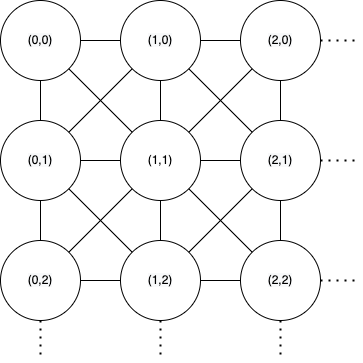
\includegraphics[scale=0.5]{pics/graph_maschen.png}
    \caption{Auschschnitt des Spielgraphen vom linken oberen \textit{Koordinatenursprung(0,0)} ausgehend.}
    \label{fig:graphMaschen}
\end{figure}